\documentclass{article}

\usepackage{graphicx}
\usepackage{tikz}
\usepackage{tikzsymbols}
\usetikzlibrary{calc,patterns,shapes.geometric}
\pagestyle{empty}
\usepackage[margin=0pt]{geometry}
\geometry{papersize={14in,12in}}

\def\centerarc[#1](#2)(#3:#4:#5){\draw[#1] ($(#2)+({#5*cos(#3)},{#5*sin(#3)})$) arc (#3:#4:#5);}

\begin{document}
	\begin{figure}
		\centering
		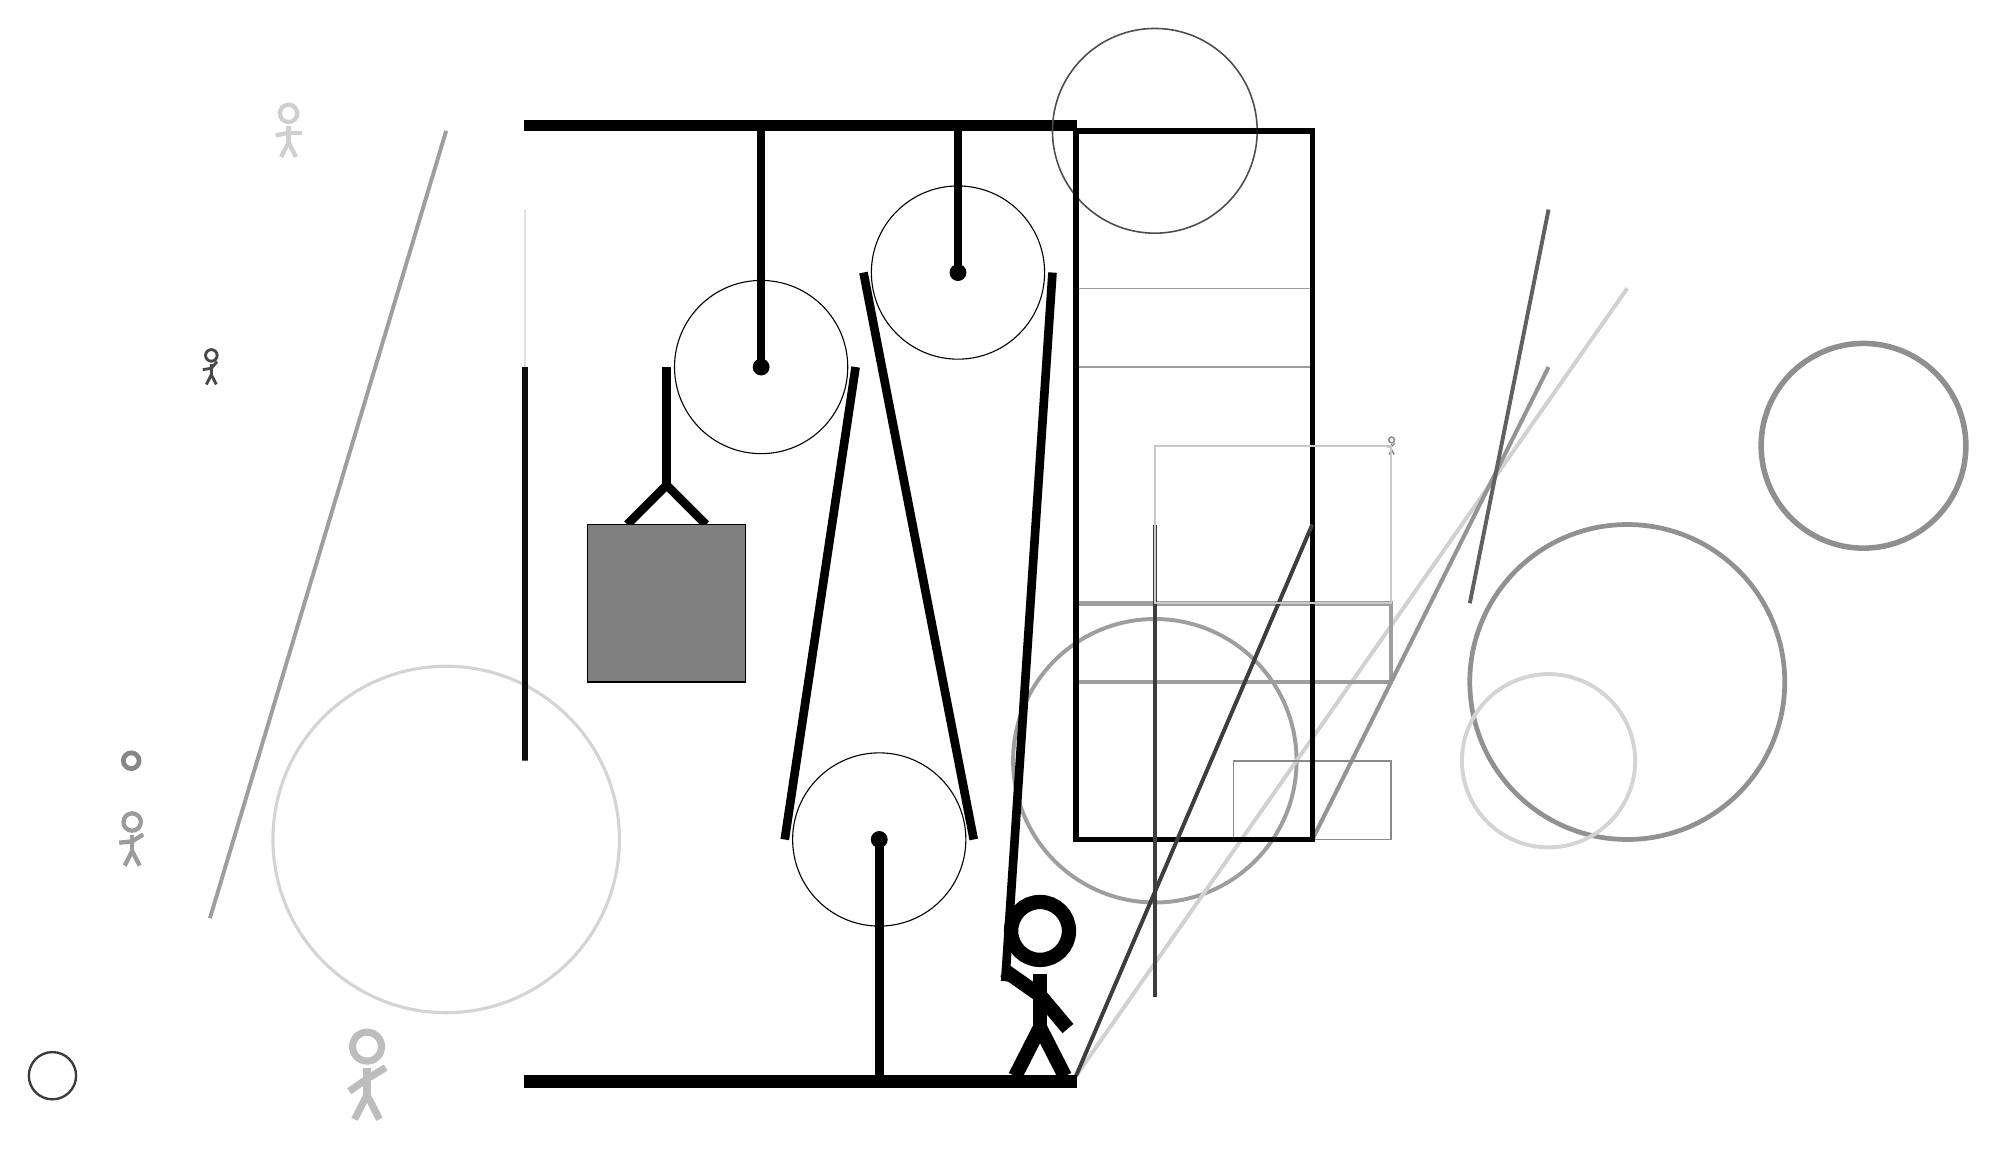
\begin{tikzpicture}
			%%%%% START %%%%%
			
			\draw[fill=black] (-2, 9) rectangle (5, 9.125);
			
			\draw[line width=0.2mm, color=black!39] (5, 6) rectangle (8, 7);
			
			\draw [line width=0.5mm, color=black!38](6, 1) circle (1.8);
			\draw [line width=0.2mm, color=black!70](6, 9) circle (1.3);
			\draw[line width=0.5mm, color=black!18](5, -3) -- (12, 7);
			\draw[line width=0.6mm, color=black!38] (5, 2) rectangle (9, 3);
			
			\draw [line width=0.6mm, color=black!43](12, 2) circle (2.0);
			\draw[line width=0.5mm, color=black!42](8, 0) -- (11, 6);
			\draw[line width=0.5mm, color=black!38](-6, -1) -- (-3, 9);
			\node[line width=0.7mm, color=black!19] at (-5, 9) {\Strichmaxerl[3][12][0]};
			
			\draw [line width=0.6mm, color=black!47](-7, 1) circle (0.1);
			
			\draw[line width=0.2mm, color=black!46] (7, 1) rectangle (9, 0);
			\draw [line width=0.3mm, color=black!77](-8, -3) circle (0.3);
			\draw[line width=0.7mm, color=black!100] (5, 0) rectangle (8, 9);
			
			\draw[line width=0.5mm, color=black!76](6, -2) -- (6, 4);
			\draw[line width=0.3mm, color=black!12] (-2, 1) rectangle (-2, 8);
			\draw [line width=0.4mm, color=black!17](-3, 0) circle (2.2);
			\draw [line width=0.5mm, color=black!17](11, 1) circle (1.1);
			\node[line width=0.5mm, color=black!26] at (-4, -3) {\Strichmaxerl[5][35][31]};
			\draw[line width=0.7mm, color=black!95] (-2, 1) rectangle (-2, 6);
			\node[line width=0.3mm, color=black!72] at (-6, 6) {\Strichmaxerl[2][9][49]};
			\draw[line width=0.5mm, color=black!76](5, -3) -- (8, 4);
			
			\node[line width=0.6mm, color=black!39] at (-7, 0) {\Strichmaxerl[3][6][32]};
			\node[line width=0.6mm, color=black!47] at (9, 5) {\Strichmaxerl[1][7][43]};
			\draw [line width=0.7mm, color=black!44](15, 5) circle (1.3);
			\draw[line width=0.5mm, color=black!62](10, 3) -- (11, 8);
			
			\draw[line width=0.2mm, color=black!21] (6, 3) rectangle (9, 5);
			
			\draw (1, 6) circle (1.1);
			\draw[fill=black] (1, 6) circle (0.1);
			\draw[line width=1.1mm]  (1, 9) -- (1, 6);
			
			\draw[fill=white](2.5, 0) circle (1.1);
			\draw[fill=black] (2.5, 0) circle (0.1);
			\draw[line width=1.1mm]  (2.5, -3) -- (2.5, 0);
			
			\draw[fill=white](3.5, 7.2) circle (1.1);
			\draw[fill=black] (3.5, 7.2) circle (0.1);
			\draw[line width=1.1mm] (3.5, 9) -- (3.5, 7.2);
			
			\draw[line width=1.1mm] (-0.7, 4.0) -- (-0.2, 4.5) -- (0.3, 4.0);
			\draw[fill=black!50] (-1.2, 4.0) rectangle (0.8, 2.0);
			
			\draw[line width=1.1mm] (-0.2, 6) -- (-0.2, 4.5);
			\centerarc[line width=1.1mm](1, 6)(0:180:1.2000000000000002);
			\draw[line width=1.1mm](2.2, 6) -- (1.3, 0);
			\centerarc[line width=1.1mm](2.5, 0)(180:360:1.2000000000000002);
			\draw[line width=1.1mm](3.7, 0) -- (2.3, 7.2);
			\centerarc[line width=1.1mm](3.5, 7.2)(0:180:1.2000000000000002);
			\draw[line width=1.1mm](4.7, 7.2) -- (4.1, -1.8);
			
			\node at (4.5, -1.9) {\Strichmaxerl[10][-35][-50]};
			
			\draw[fill=black] (-2, -3) rectangle (5, -3.15);
			
			%%%%% END %%%%%
		\end{tikzpicture}
	\end{figure}	
\end{document}